\resizebox{\columnwidth}{!}{
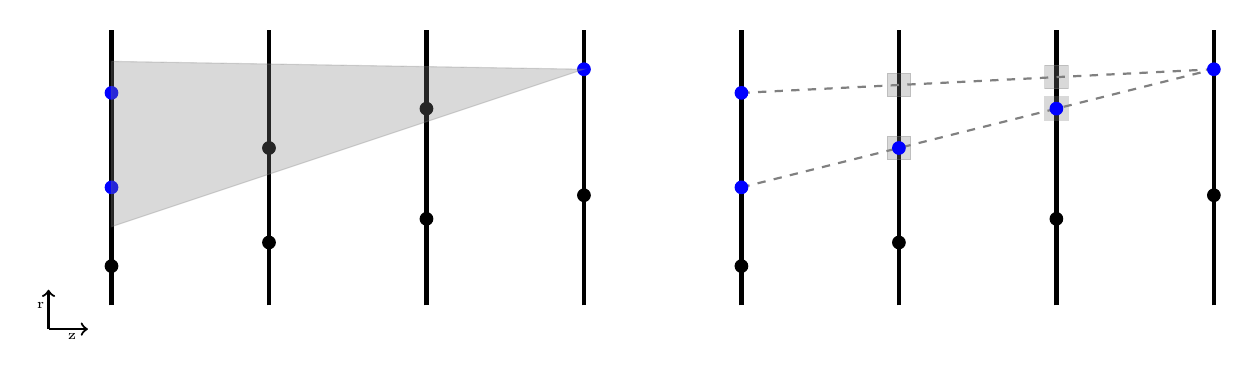
\begin{tikzpicture}
  %\draw[step=1cm,gray,very thin] (0,0) grid (15,4.5);
  \draw[ultra thick] (1.,0.5) -- (1.,4);
  \draw[ultra thick] (3,0.5) -- (3,4);
  \draw[ultra thick] (5,0.5) -- (5,4);
  \draw[ultra thick] (7,0.5) -- (7,4);
  
  \draw[fill,blue] (7,3.5) circle (0.08);
  \draw[fill,blue] (1,2) circle (0.08);
  \draw[fill] (3,2.5) circle (0.08);
  \draw[fill] (5,3) circle (0.08);
  
  \draw[fill] (1,1.) circle (0.08);
  \draw[fill] (3,1.3) circle (0.08);
  \draw[fill] (5,1.6) circle (0.08);
  \draw[fill] (7,1.9) circle (0.08);
  
  \draw[fill,blue] (1,3.2) circle (0.08);
  
  \draw[fill,gray,opacity=0.3] (7,3.5)--(1,1.5)--(1,3.6)--cycle;
  
  \draw[ultra thick] (9.,0.5) -- (9.,4);
  \draw[ultra thick] (11,0.5) -- (11,4);
  \draw[ultra thick] (13,0.5) -- (13,4);
  \draw[ultra thick] (15,0.5) -- (15,4);
  
  \draw[thick,gray, dashed] (9,2) -- (15,3.5);
  \draw[thick,gray, dashed] (9,3.2) -- (15,3.5);
  
  \draw[fill,gray,opacity=0.3] (10.85,2.35) rectangle (11.15,2.65);
  \draw[fill,gray,opacity=0.3] (12.85,2.85) rectangle (13.15,3.15);
  
  \draw[fill,gray,opacity=0.3] (10.85,3.15) rectangle (11.15,3.45);
  \draw[fill,gray,opacity=0.3] (12.85,3.25) rectangle (13.15,3.55);
  
  \draw[fill,blue] (15,3.5) circle (0.08);
  \draw[fill,blue] (9,2) circle (0.08);
  \draw[fill,blue] (11,2.5) circle (0.08);
  \draw[fill,blue] (13,3) circle (0.08);
  
  \draw[fill] (9,1.) circle (0.08);
  \draw[fill] (11,1.3) circle (0.08);
  \draw[fill] (13,1.6) circle (0.08);
  \draw[fill] (15,1.9) circle (0.08);
  
  \draw[fill,blue] (9,3.2) circle (0.08);
  
  \draw[thick,->] (0.2,0.2) -- (0.7,0.2);
  \draw[thick,->] (0.2,0.2) -- (0.2,0.7);
  
  \node[draw=none] at (0.5,0.1){\tiny z};
  \node[draw=none] at (0.1,0.5){\tiny r};
  
\end{tikzpicture}
}